%=========================================================================
%  IEEEtran two-column version (conference / capstone report).
%  The journal version is main.tex. Both include abstract.tex and body.tex.
%  Overleaf: upload the whole paper/ folder plus figures/ (next to the .tex
%  files). Compiler: pdfLaTeX. Set main_ieee.tex as the main document.
%=========================================================================
\documentclass[conference]{IEEEtran}
\IEEEoverridecommandlockouts
\usepackage{cite}
\usepackage{amsmath,amssymb,amsfonts}
\usepackage{graphicx}
\usepackage{booktabs}
\usepackage{multirow}
\usepackage{xcolor}
\usepackage[hidelinks]{hyperref}

\graphicspath{{./}{../}}   % figures/ next to the .tex files (Overleaf) or at the repo root
% Generated by scripts/make_paper_assets.py from results/final/ -- do not edit by hand.
\newcommand{\nPPOx}{3.9}
\newcommand{\nPPOxLo}{3.0}
\newcommand{\nPPOxHi}{5.1}
\newcommand{\nPPOseedMin}{2.6}
\newcommand{\nPPOseedMax}{5.3}
\newcommand{\nPPOdisp}{12.3}
\newcommand{\nORdisp}{2.78}
\newcommand{\nPPOlat}{0.0477}
\newcommand{\nPPOrec}{0.0672}
\newcommand{\nORlat}{0.0537}
\newcommand{\nUNIlat}{0.0455}
\newcommand{\nEWMAlat}{0.0548}
\newcommand{\nEWMArec}{0.0595}
\newcommand{\nEWMAx}{1.41}
\newcommand{\nRFx}{1.36}
\newcommand{\nUNIx}{0.36}
\newcommand{\nPPOgap}{0.0196}
\newcommand{\nEWMAgap}{0.0047}
\newcommand{\nORgap}{0.0030}
\newcommand{\nPPOrd}{1.89}
\newcommand{\nORrd}{1.58}
\newcommand{\nEWMArd}{1.75}
\newcommand{\nPPOvsEWMA}{2.8}
\newcommand{\nPPOORx}{1.22}
\newcommand{\nPPOORlat}{0.0490}
\newcommand{\nBRRx}{13.0}
\newcommand{\nBRRrec}{0.0746}
\newcommand{\nBRRlat}{0.0475}
\newcommand{\nBRLx}{2.2}
\newcommand{\nBRLlat}{0.0552}
\newcommand{\nAttRecRec}{4.85}
\newcommand{\nAttLatRec}{2.20}
\newcommand{\nAttRecLat}{1.38}
\newcommand{\nAttLatLat}{1.20}
\newcommand{\nPPOcoef}{3.8}
\newcommand{\nPPOt}{7.8}
\newcommand{\nPPOseedsPos}{5/5}
\newcommand{\nPPOcoefLo}{2.0}
\newcommand{\nPPOcoefHi}{5.6}
\newcommand{\nBRRcoef}{10.3}
\newcommand{\nPtwoCoef}{-12.0}
\newcommand{\nPtwox}{0.66}
\newcommand{\nPtwolat}{0.0481}
\newcommand{\nPfourx}{0.11}
\newcommand{\nPfourlat}{0.0339}
\newcommand{\nRfivex}{2.98}
\newcommand{\nRonefivex}{0.76}
\newcommand{\nRonefivelat}{0.0490}
\newcommand{\nRonefiveLo}{0.69}
\newcommand{\nRonefiveHi}{0.85}
\newcommand{\nRhalfx}{0.53}
\newcommand{\nRonefiveLatP}{0.005}
\newcommand{\nEfiveBase}{4.9}
\newcommand{\nEfiveBaseLo}{4.1}
\newcommand{\nEfiveBaseHi}{5.9}
\newcommand{\nEfivePerf}{1.65}
\newcommand{\nEfiveConst}{1.46}
\newcommand{\nEfiveConstLo}{1.36}
\newcommand{\nEfiveConstHi}{1.59}
\newcommand{\nEfiveFairMin}{0.33}
\newcommand{\nEfiveFairMax}{0.36}
\newcommand{\nPPObeta}{3.1}
\newcommand{\nPPOw}{+1.28}
\newcommand{\nPPOmu}{0.14}
\newcommand{\nNContrasts}{19}
\newcommand{\nPPOsis}{0.48}
\newcommand{\nORsis}{0.51}
\newcommand{\nEWMAsis}{0.61}
\newcommand{\nPPOqfive}{+27}
\newcommand{\nPPOqtwothree}{-10}
\newcommand{\nORqfive}{-5}
\newcommand{\nEWMAqfive}{-2}

% Generated by scripts/make_journal_assets.py -- do not edit by hand.
\newcommand{\nThEpsBase}{+0.20}
\newcommand{\nThEpsConst}{-0.35}
\newcommand{\nThEpsDetect}{0.55}
\newcommand{\nThEpsDeter}{0.35}
\newcommand{\nThBetaCrit}{5.0}
\newcommand{\nThAmpOne}{1.25}
\newcommand{\nThAmpConstOne}{0.74}
\newcommand{\nThRtwo}{0.98}
\newcommand{\nThDispErr}{2}
\newcommand{\nThDispErrMax}{7}
\newcommand{\nThNrules}{24}
\newcommand{\nThLamRatio}{4.5}
\newcommand{\nThBetaRecBase}{4}
\newcommand{\nThBetaLatBase}{1.5}
\newcommand{\nThBetaRecConst}{2}
\newcommand{\nThSimBaseFour}{7.4}
\newcommand{\nThModBaseFour}{6.4}
\newcommand{\nThSimConstFour}{3.2}
\newcommand{\nThModConstFour}{3.0}
\newcommand{\nThSimBaseOne}{1.40}
\newcommand{\nThSimConstOne}{0.99}
\newcommand{\nThRecGainBase}{17}
\newcommand{\nThRecGainConst}{2}
\newcommand{\nThConstBetaOneFiveX}{1.4}
\newcommand{\nThConstFlat}{0.8}
\newcommand{\nRefUniPPO}{10.8}
\newcommand{\nRefEwmaPPO}{2.8}
\newcommand{\nRefBrlPPO}{1.7}
\newcommand{\nTopPPO}{2.75}
\newcommand{\nTopPPOLo}{2.45}
\newcommand{\nTopPPOHi}{3.04}
\newcommand{\nTopOR}{0.96}
\newcommand{\nTopEWMA}{1.11}
\newcommand{\nTopBRR}{4.18}
\newcommand{\nTopBRL}{1.34}
\newcommand{\nTopUNI}{0.55}
\newcommand{\nTopTarget}{0.98}
\newcommand{\nTvPPO}{0.38}
\newcommand{\nTvOR}{0.02}
\newcommand{\nTvUNI}{0.24}
\newcommand{\nLongX}{3.9}
\newcommand{\nLongXLo}{3.2}
\newcommand{\nLongXHi}{4.6}
\newcommand{\nLongRec}{0.0680}
\newcommand{\nLongLat}{0.0472}
\newcommand{\nThreeX}{4.8}
\newcommand{\nThreeRec}{0.0689}
\newcommand{\nCurveRecStart}{0.0616}
\newcommand{\nCurveRecEnd}{0.0677}
\newcommand{\nCurveXStart}{2.6}
\newcommand{\nCurveXMid}{5.3}
\newcommand{\nCurveXEnd}{4.2}
\newcommand{\nHpXMin}{2.3}
\newcommand{\nHpXMax}{8.2}
\newcommand{\nHpLoMin}{2.0}
\newcommand{\nHpRecMax}{0.0722}
\newcommand{\nHpLatMax}{0.0485}
\newcommand{\nHpN}{20}
\newcommand{\nCurveRecMid}{0.0687}
\newcommand{\nHpRecMin}{0.0629}
\newcommand{\nHpLatMin}{0.0472}
\newcommand{\nBestModelRec}{0.0741}
\newcommand{\nBestModelX}{12.0}
\newcommand{\nHpRho}{0.96}
\newcommand{\nHpRhoP}{<0.001}
\newcommand{\nSnapRho}{0.90}
\newcommand{\nSnapN}{36}
\newcommand{\nLagX}{1.04}
\newcommand{\nLagXLo}{0.90}
\newcommand{\nLagXHi}{1.18}
\newcommand{\nLagLat}{0.0460}
\newcommand{\nSensMin}{3.2}
\newcommand{\nSensMax}{9.1}
\newcommand{\nSensLoMin}{2.62}
\newcommand{\nSensN}{7}
\newcommand{\nSensRho}{0.93}
\newcommand{\nSensRhoP}{0.003}
\newcommand{\nSensBase}{4.9}
\newcommand{\nSensLowDetectGain}{3.5}
\newcommand{\nSensHighDetectGain}{5.6}
\newcommand{\nSensLowPReport}{8.1}
\newcommand{\nSensHighPReport}{3.2}
\newcommand{\nSensWeakDeterrence}{9.1}
\newcommand{\nSensStrongDeterrence}{5.5}
\newcommand{\nSensNoSocioObs}{4.4}
\newcommand{\nEpsLowDetectGain}{+0.01}
\newcommand{\nEpsHighDetectGain}{+0.29}
\newcommand{\nEpsLowPReport}{+0.36}
\newcommand{\nEpsHighPReport}{+0.07}
\newcommand{\nEpsWeakDeterrence}{+0.44}
\newcommand{\nEpsStrongDeterrence}{+0.12}

% \input is not expandable, which breaks \bottomrule after a table body; use the primitive
\makeatletter\newcommand{\tabinput}[1]{\@@input #1.tex }\makeatother
\newenvironment{widefigure}{\begin{figure*}[t]\centering}{\end{figure*}}
\newenvironment{widetable}{\begin{table*}[t]\centering}{\end{table*}}
\newenvironment{landtable}{\begin{table*}[t]\centering}{\end{table*}}
\newsavebox{\fitboxbox}
\newenvironment{fitbox}{\begin{lrbox}{\fitboxbox}}{\end{lrbox}%
  \ifdim\wd\fitboxbox>\linewidth \resizebox{\linewidth}{!}{\usebox{\fitboxbox}}%
  \else \usebox{\fitboxbox}\fi}   % shrink a table only if it is wider than the column
\newcommand{\archwidth}{0.82\textwidth}
\newcommand{\widefigwidth}{0.9\textwidth}
\newcommand{\narrowfigwidth}{\linewidth}

\begin{document}

\title{Optimising a Self-Contaminated Proxy:\
Patrol-Allocation Bias in a Crime Simulator\
with Known Ground Truth}

\author{
\IEEEauthorblockN{Ashmith Reddy Sama, Dennis Philip, Dhrithi Kiran, Diya Saigal}
\IEEEauthorblockA{Department of Computer Science and Engineering (AI \& ML)\
PES University, Bengaluru, India}
\and
\IEEEauthorblockN{Bhaskarjyoti Das}
\IEEEauthorblockA{Department of Computer Science and Engineering (AI \& ML)\
PES University, Bengaluru, India}
}

\maketitle

\begin{abstract}
A system that acts on the world and is then scored on what it observes can write
part of its own objective. In patrol allocation, patrolling a district raises
the fraction of its crime that is recorded, and recorded crime is both the input
and the success measure of the next allocation. We study what happens when such
a \emph{self-contaminated proxy} is optimised, using an agent-based crime
simulator that is never seeded with historical crime, so latent crime is known
everywhere. Policies set the parameters of an allocation rule and are rewarded
for covering \emph{recorded} crime; each is scored against a need-proportional
reference on the same simulator seeds. A reinforcement-learning agent (PPO)
places \nPPOx$\times$ the reference's patrol disparity on the most disadvantaged
districts (95\% CI \nPPOxLo--\nPPOxHi) while covering less true crime than the
reference, and a non-learning search that maximises the same proxy is more
skewed still (\nBRRx$\times$): the bias belongs to the objective, and better
optimisation makes it worse. A mean-field model of the loop explains why.
Patrol-dependent recording makes the recorded signal rise with patrol, which
amplifies the tilt of any allocation rule and keeps the proxy reward increasing
with concentration after true-crime coverage has peaked; the model reproduces
the simulator's disparities to within \nThDispErr\% on average. Removing the
dependence of detection on patrol cuts PPO's excess from \nEfiveBase$\times$ to
\nEfiveConst$\times$. Parity penalties overcorrect and under-patrol the
districts with the most crime, whereas a penalty targeted at the
need-proportional reference lands closest to it while raising true-crime
coverage.

\end{abstract}

\begin{IEEEkeywords}
feedback loops, proxy objectives, reinforcement learning, performative
prediction, algorithmic fairness, predictive policing, agent-based simulation
\end{IEEEkeywords}

%=========================================================================
%  Class-independent body of the paper. Included by
%      main.tex       Springer Nature (sn-jnl) journal version
%      main_ieee.tex  IEEEtran two-column version
%  The wrappers define the widefigure / widetable environments and \tabinput.
%
%  Every number comes from numbers.tex / numbers_journal.tex and every table
%  body from tables/*.tex, generated by
%      scripts/summarise_400k.py        scripts/make_paper_assets.py
%      scripts/reference_robustness.py  scripts/analytic_model.py
%      scripts/summarise_journal.py     scripts/make_journal_assets.py
%  Do not type numbers by hand; regenerate instead.
%=========================================================================

\section{Introduction}

When a model's outputs change the data it is later trained and judged on, the
data are no longer exogenous. Performative prediction~\cite{perdomo2020}
formalises this for supervised learning, the selective-labels
problem~\cite{lakkaraju2017} shows how a decision can censor the outcomes needed
to evaluate it, and Goodhart's law~\cite{manheim2018} names the general failure:
a measure that is optimised stops measuring. The coupling is tightest when the
optimiser acts repeatedly and its actions change what is \emph{observed}, not
only what happens. The objective is then a proxy that the optimiser partly
writes itself. We call such a proxy \emph{self-contaminated}.

Patrol allocation is the canonical example. An officer present in an area
discovers more of the crime that happens there, so sending patrols raises an
area's \emph{recorded} crime even when its \emph{true} rate is unchanged; the
higher record then justifies the allocation. Ensign et al.~\cite{ensign2018}
formalised this loop with urn models, and Lum and Isaac~\cite{lum2016} traced
its consequences on Oakland drug-crime data. Two things are hard to get in that
setting. The true crime rate is unobserved, so an allocation cannot be scored
against where crime actually is. And the allocators studied follow a fixed
update, so the question of what an \emph{optimiser} does with such a signal --
a tuned heuristic, a search procedure or a reinforcement-learning (RL) agent
rewarded for ``being where crime is found'' -- is left open.

We supply both. Our environment is an agent-based model (ABM) of urban violent
crime whose risk surface starts spatially flat and into which no historical crime
coordinates are ever injected, so the latent crime count of each of Chicago's 22
police districts is known in every shift. Around it we close the loop
(Fig.~\ref{fig:arch}): a policy sets the parameters of an allocation rule over
recorded crime, patrol raises detection, and the policy is rewarded for covering
recorded crime. Because high-hardship districts have more latent crime, raw
enforcement disparity mixes legitimate targeting with bias. We therefore measure
each policy against a \emph{need-proportional reference} that allocates in
proportion to latent crime, paired on the same simulator seed.

Three optimisers of the same proxy are compared: a PredPol-style heuristic that
does not optimise at all, a PPO agent, and an exhaustive search over the rule
class. The further the proxy is optimised, the larger the bias. A mean-field
model of the loop shows that this is not an accident of the learner: when
detection rises with patrol, the proxy reward keeps increasing with
concentration after true-crime coverage has started to fall, and the loop
multiplies whatever tilt the rule intends.

\begin{widefigure}
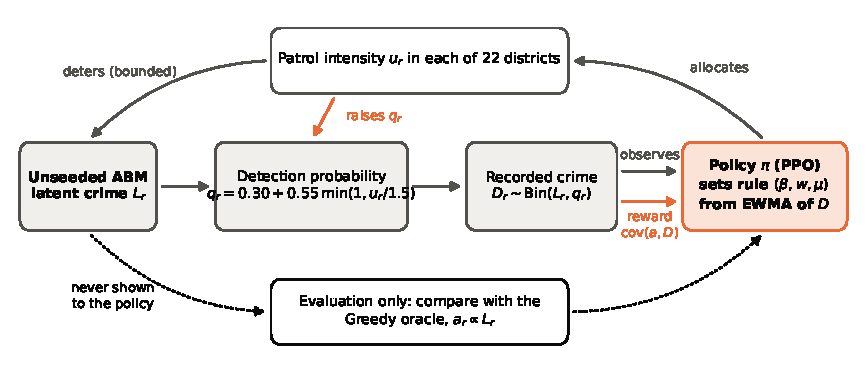
\includegraphics[width=\archwidth]{figures/fig_arch.pdf}
\caption{The closed loop. Latent crime $L_r$ is thinned into recorded crime
$D_r$ with a detection probability that rises with patrol intensity $u_r$. The
policy observes only recorded crime and is rewarded for covering it. Latent
crime is used only for evaluation, through the need-proportional reference.}
\label{fig:arch}
\end{widefigure}

We ask:
\begin{itemize}
\item[\textbf{E1}] How far from the need-proportional reference does an
optimiser of recorded-crime coverage move enforcement, what does it cost in
true-crime coverage, and does the answer depend on how well the proxy is
optimised?
\item[\textbf{E2}] Does the policy contaminate its own objective?
\item[\textbf{E3}] Does the excess fall on disadvantaged districts once their
latent need is controlled for?
\item[\textbf{E4}] Can a penalty remove the excess without overcorrecting?
\item[\textbf{E5}] How much of the excess disappears when patrol no longer
changes detection, and how sensitive is it to the detection and deterrence
parameters?
\end{itemize}

\noindent\textbf{Contributions.}
(1)~A closed-loop testbed with known ground truth in which a policy's
observations and reward are contaminated by its own actions, released as a
Gymnasium environment.
(2)~A reference-relative bias measure (paired log-ratio to a need-proportional
allocation, with a hierarchical bootstrap over training and evaluation seeds)
that separates excess concentration from legitimate targeting, with a proof
that orderings and contrasts do not depend on the reference and two
reference-free checks.
(3)~A mean-field model of the loop that gives the amplification factor
$1/(1-\beta\varepsilon)$ in closed form, predicts the simulator's disparities
within \nThDispErr\% on average, and explains why the proxy optimum is more
concentrated than the true optimum.
(4)~An attribution of the excess across optimisers (heuristic, RL, exhaustive
search), across what the agent observes and is rewarded on, and across the
detection channel, which locates the bias in the proxy objective rather than in
RL.
(5)~Evidence that parity penalties overcorrect, and a penalty targeted at the
reference that gets closer to it while raising true-crime coverage.

\section{Related Work}

\textbf{Performative, selectively labelled and gamed signals.}
Perdomo et al.~\cite{perdomo2020} study predictions that influence the outcomes
they forecast and characterise when repeated retraining converges. Lakkaraju et
al.~\cite{lakkaraju2017} show that when a decision determines which outcomes are
observed, naive evaluation is biased. Manheim and
Garrabrant~\cite{manheim2018} classify the ways in which optimising a metric
breaks its relation to the goal. Our setting combines all three: the action
changes which crimes are recorded, the record is the optimisation target, and
the optimiser acts every shift.

\textbf{Feedback loops in predictive policing.}
Ensign et al.~\cite{ensign2018} model discovered-incident feedback with P\'olya
urns, prove that the allocation can run away to a single area, and give
black-box corrections. Lum and Isaac~\cite{lum2016} show the disparate impact
empirically, and Akpinar et al.~\cite{akpinar2021} show that differential
victim reporting alone biases hot-spot prediction. A simulation study of
predictive versus hot-spots policing in Baltimore~\cite{algorithms2026} finds
the predictive system faster to amplify bias. We differ in three ways: latent
crime is known, so bias is measured against need rather than inferred; the
allocation rule is \emph{optimised} for the contaminated signal rather than
fixed; and detection saturates and patrol deters, which turns runaway into a
bounded amplification that we characterise.

\textbf{Long-term fairness in simulation.}
D'Amour et al.~\cite{damour2020} and Liu et al.~\cite{liu2018} show that
fairness criteria evaluated on a static snapshot can harm the protected group
once the environment responds, and FairSense~\cite{fairsense2025} simulates
long-term fairness of ML-enabled systems in general. Our parity-penalty result
is an instance: a constraint that ignores need under-patrols the districts with
the most crime.

\textbf{RL for patrol allocation.}
Repasky et al.~\cite{repasky2024} treat each patrol unit as a Q-learner; the
cooperative-routing model of~\cite{jocv2025} maximises coverage of historical
crime with a decentralised POMDP; and~\cite{ceus2025} uses deep RL to solve a
maximum-coverage design problem with a regional-disparity constraint. All three
optimise coverage of a fixed signal; the policy's actions do not enter its data.

\textbf{Constrained and fair RL; crime ABMs.}
Our penalties follow the constrained-MDP literature~\cite{chow2017,
tessler2019, stooke2020}, and the exposure constraint follows demographic parity
in sequential decisions~\cite{dwork2012, jabbari2017}. Wise and
Cheng~\cite{wise2024} give offender agents RL; we keep offenders rule-based.
Our generator continues data-driven and routine-activity crime
ABMs~\cite{roses2021, palma2025, caresim2023}; the distinguishing choice is the
flat, unseeded risk surface.

\section{The Emergent Crime Simulator}

A $20\times20$ grid overlays Chicago; each cell takes its modal police district,
giving 22 districts as the unit of allocation and fairness. District covariates
are aggregated from the community-area American Community Survey hardship table.
Residential population is treated as uniform across districts, so per-capita
crime is emergent rather than an input. $N=200$ agents have a home district $r$,
employment at the district unemployment rate, and stress
$s_i = s_0 + h_r + \epsilon_i$ with hardship $h_r\in[0,1]$,
$\epsilon_i\sim\mathcal{U}(0,0.2)$ and $s_0=0.2$. They move on routine-activity
schedules (work 9--17, leisure 18--23, home otherwise).

The environmental risk grid starts at a uniform constant, and \emph{no historical
crime coordinates enter it at any point}; it decays and grows with local
occupancy. An agent commits a violent act through an environmental path, when a
smoothed risk combining stress, local risk and a mean-field escalation term
exceeds a threshold, or through an interaction path whose rate rises with nearby
high-stress agents~\cite{roses2021}. One shift is four sub-steps and yields the
latent violent-crime count per district, $L_r$. The vectorised generator passes
the calibration gate of the earlier Mesa model: crime rises with hardship
(by 27\% from low- to high-hardship scenarios), monotonically across
three scenarios, clusters spatially from the flat start, and is higher at night.

\section{Closed-Loop Allocation and Measurement}

\subsection{Action: rule parameters}
The environment keeps an exponentially weighted moving average $\bar D_r$ of
recorded crime (half-life 5 shifts). An action $(\beta, w, \mu)$ gives the
deployment share
\begin{equation}
a_r \;\propto\; (1-\mu)\,
\frac{(\bar D_r/\overline{\bar D})^{\beta}\, e^{\,w\, z_r}}
{\sum_{r'} (\bar D_{r'}/\overline{\bar D})^{\beta}\, e^{\,w\, z_{r'}}}
\;+\; \frac{\mu}{22},
\label{eq:rule}
\end{equation}
with $z_r$ the standardised district hardship, $\beta\in[0,4]$ the concentration
on recorded crime, $w\in[-2,2]$ an explicit hardship tilt and $\mu\in[0,1]$ a
uniform mix, plus a floor of $0.005$ per district. The rule always reads
\emph{recorded} crime; giving the policy latent crime changes its observation,
not the rule's input. A PredPol-style heuristic~\cite{ensign2018} is the rule
with $(\beta, w, \mu) = (1, 0, 0)$. The rule class is deliberately small: it can
be searched exhaustively, which lets us compare a learner with the true optimum
of its own objective.

\subsection{Transition and self-contaminated observation}
With patrol intensity $u_r$ relative to a proportional allocation, deterrence
removes $\min(0.68, 0.26\,u_r)$ of latent crime~\cite{weisburd2017}, and the
recorded count is a thinning
\begin{equation}
D_r \sim \mathrm{Binomial}(L_r,\, q_r), \qquad
q_r = 0.30 + 0.55\,\min(1, u_r/1.5).
\label{eq:detect}
\end{equation}
The observation kernel $P(D \mid L, u)$ therefore depends on the policy's own
action: this is the contamination. Under uniform patrol $q_r = 0.667$ everywhere.
The policy observes $\bar D$, its last deployment, time of day and static district
covariates, never $L$.

\subsection{Objectives and policies}
With $\mathrm{cov}(a, X) = \sum_r a_r X_r / \sum_r X_r$, the reward is the
recorded coverage $\mathrm{cov}(a, D)$, the operational criterion of predictive
policing. We report it alongside the true-crime coverage $\mathrm{cov}(a, L)$.
The learner is PPO~\cite{schulman2017ppo, sb3} with a two-layer MLP, trained for
400k steps on randomly seeded episodes of 140 shifts. Baselines: Uniform, Random,
PredPol (EWMA), a random-forest hotspot model refit every 15 shifts, and the
\emph{greedy oracle}, $a_r \propto \bar L_r$, which is not deployable. Two
penalised families subtract a cost from the reward each shift:
\begin{align}
\text{parity:}\quad & w\,\delta_t, \\
\text{oracle-targeted:}\quad & w\,\max\!\big(0,\ \ln\delta_t - \ln\delta_{\mathrm{ref}}\big),
\end{align}
where $\delta_t$ is the per-shift disparity defined below and
$\delta_{\mathrm{ref}} = \nORdisp$ is the greedy oracle's mean per-shift
disparity on reference seeds 1000--1009, disjoint from every evaluation seed.

\subsection{Measuring bias relative to need}
\label{sec:measure}
Districts are split into hardship quintiles of 4--5 districts. The
\emph{disparity} $\delta$ of an episode is the mean patrol exposure per capita in
the most disadvantaged quintile divided by that in the least disadvantaged. High
hardship districts do have more latent crime, so $\delta>1$ is not by itself a
bias. We take the greedy oracle as a \emph{normative reference} -- patrol in
proportion to need -- and report, for policy $\pi$ on evaluation seed $e$,
\begin{equation}
\Delta_{\pi,e} = \ln\delta_{\pi,e} - \ln\delta_{\mathrm{oracle},e},
\qquad
\times\text{oracle} = \exp\big(\overline{\Delta}\big),
\label{eq:dlog}
\end{equation}
a geometric-mean ratio paired on the evaluation seed. 95\% confidence intervals
come from a hierarchical bootstrap (4000 replicates) that resamples training
seeds and then evaluation seeds, keeping evaluation seeds paired across policies.
The reference is not an efficiency bound: the best fixed rule for true-crime
coverage beats it (\nBRLlat{} vs \nORlat) at \nBRLx$\times$ its disparity. We
also report the \emph{proxy gap} $\mathrm{cov}(a,D)-\mathrm{cov}(a,L)$ and the
\emph{over-recording ratio}: the recorded-to-latent crime share in the top
hardship quintile divided by the same in the bottom quintile.

\textbf{Invariance to the reference.} Because~\eqref{eq:dlog} subtracts the same
per-seed term from every policy, replacing the oracle by any other reference
policy $\rho$ changes every $\overline\Delta$ by the same constant
$\overline{\ln\delta_{\mathrm{oracle}} - \ln\delta_\rho}$. The ordering of
policies, every paired contrast and every bootstrap $p$-value are therefore
identical under any reference; only the position of ``1'' moves.
Section~\ref{sec:reference} shows how far, and adds two measures that use no
reference policy at all.

\textbf{Evaluation protocol.} The main experiments use 5 training seeds (0--4)
and 30 held-out evaluation seeds (200--229). The $2\times2$ cells and the
oracle-targeted penalty use training seeds 0--2. E5 and the sensitivity analysis
use 3 training seeds and 20 evaluation seeds (300--319), each setting against
its own oracle. Pairwise comparisons use the same bootstrap and two-sided
bootstrap $p$-values, Holm-adjusted over all \nNContrasts{} pre-specified
contrasts (Table~\ref{tab:contrasts}).

\section{A Mean-Field Model of the Loop}
\label{sec:model}

Before the experiments we ask what a rule of the form~\eqref{eq:rule} does in
steady state when its input depends on its output. Replace counts by their means
and let district $r$ have untreated crime rate $\lambda_r$ and population share
$\pi_r$. With the budget at its reference level, a patrol share $a_r$ gives
intensity $u_r = a_r/\pi_r$, and
\begin{equation}
\begin{gathered}
L_r = \lambda_r\,\kappa(u_r), \qquad \bar D_r = L_r\, q(u_r), \\
\kappa(u) = 1 - \min(0.68,\, 0.26\,u),
\end{gathered}
\end{equation}
with $q$ from~\eqref{eq:detect}. Write $h(u) = q(u)\,\kappa(u)$ for the factor by
which patrol scales the signal the rule reads ($h=\kappa$ for a rule that reads
latent crime, such as the oracle). A steady state of the rule with $\mu=0$ is a
fixed point
\begin{equation}
a_r \;=\; \frac{1}{Z}\,\big[\lambda_r\, h(a_r/\pi_r)\big]^{\beta}\, e^{\,w z_r},
\qquad \textstyle\sum_r a_r = 1 .
\label{eq:fp}
\end{equation}
Let $\varepsilon(u) = \mathrm{d}\ln h/\mathrm{d}\ln u$ be the elasticity of the
signal to patrol. For recorded crime below the saturation points,
\begin{equation}
\varepsilon(u) \;=\;
\underbrace{\frac{0.55\,u/1.5}{0.30 + 0.55\,u/1.5}}_{\text{detection}}
\;-\;
\underbrace{\frac{0.26\,u}{1 - 0.26\,u}}_{\text{deterrence}} ,
\label{eq:eps}
\end{equation}
which is $\nThEpsDetect - \nThEpsDeter = \nThEpsBase$ at proportional patrol
($u=1$). If detection does not depend on patrol only the second term remains
and $\varepsilon = \nThEpsConst$.

\textbf{Proposition 1 (amplification).} Suppose $\pi_r$ is uniform and
$\ln h$ is linear in $\ln u$ with slope $\varepsilon$ over the intensities in
use. If $\beta\varepsilon < 1$, the fixed point~\eqref{eq:fp} is unique and
\begin{equation}
\ln a_r \;=\; \frac{\beta \ln\lambda_r + w\,z_r}{1-\beta\varepsilon} + c ,
\label{eq:amp}
\end{equation}
with $c$ fixed by normalisation; it is locally stable under the EWMA update.
If $\beta\varepsilon > 1$ the interior fixed point is unstable and the
allocation moves to the boundary.

\emph{Proof.} Taking logarithms of~\eqref{eq:fp} and substituting
$\ln h(a_r/\pi_r) = \ln h_0 + \varepsilon \ln a_r$ gives
$\ln a_r = \beta\ln\lambda_r + \beta\varepsilon\ln a_r + w z_r + c'$, which
solves to~\eqref{eq:amp} when $\beta\varepsilon \neq 1$. In log-shares the
update map has slope $\beta\varepsilon$ in every direction tangent to the
simplex; with EWMA weight $\eta\in(0,1]$ on the new signal the linearised
iteration has multiplier $1-\eta+\eta\beta\varepsilon$, which lies in $(-1,1)$
when $\beta\varepsilon<1$ (and $\beta\varepsilon > 1-2/\eta$, which holds for
every setting here). For $\beta\varepsilon>1$ the multiplier exceeds 1.
\hfill$\square$

Three consequences follow. \emph{(i) The loop is a multiplier.} A rule intends
the tilt $\beta\ln\lambda_r + w z_r$; the loop delivers $1/(1-\beta\varepsilon)$
times it. A proportional rule ($\beta=1$) on recorded crime is amplified by
$\nThAmpOne$, while the same rule on a signal with patrol-independent detection,
or the oracle reading latent crime, is \emph{damped} to $\nThAmpConstOne$,
because deterrence lowers crime where patrol goes. Recorded-crime allocation is
thus more concentrated than need-proportional allocation even with no optimiser
in the loop. \emph{(ii) Amplification is bounded.} Runaway to a single district,
as in the urn model of~\cite{ensign2018}, needs $\beta\varepsilon>1$, i.e.\
$\beta > \nThBetaCrit$ at $u=1$, outside the rule's range. Moreover
$\varepsilon(u)$ falls with $u$ and turns negative once detection saturates
($u>1.5$): districts that attract patrol stop looking worse. A saturating
detection curve converts runaway into a finite excess. \emph{(iii) The proxy
rewards concentration.} For a fixed record the reward
$\mathrm{cov}(a,D)=\sum_r a_r D_r/\sum_r D_r$ is linear in $a$ and is maximised
by putting all patrol on the district with the largest record; what limits
concentration is only the response of $D$ to $a$. When $\varepsilon>0$ that
response favours the optimiser (patrol raises the record share of the district
it is sent to), and when $\varepsilon<0$ it penalises it. The proxy optimum is
therefore more concentrated than the true-coverage optimum, whose signal
elasticity is $\nThEpsConst$.

\textbf{Check against the simulator.} We solve~\eqref{eq:fp} numerically with
the exact piecewise $q$ and $\kappa$, the floor, and $\lambda_r$ estimated once
from a uniform-patrol rollout (the top hardship quintile has \nThLamRatio$\times$
the untreated crime of the bottom one). We then roll out fixed rules with
$w=\mu=0$ and $\beta\in\{0.5,\dots,4\}$ in the full agent-based simulator, with
and without patrol-dependent detection, on seeds disjoint from all evaluation
seeds (Fig.~\ref{fig:theory}). Over the \nThNrules{} rule--setting pairs the
model's disparity is within \nThDispErr\% of the simulator's on average (at most
\nThDispErrMax\%), and it explains \nThRtwo{} of the variance of the log
disparity relative to the oracle. At $\beta=4$ the same rule sits at
\nThSimBaseFour$\times$ the oracle with the recording loop and
\nThSimConstFour$\times$ without it (model: \nThModBaseFour{} and
\nThModConstFour). In the base setting recorded coverage rises monotonically
with $\beta$ up to the edge of the rule class, \nThRecGainBase\% above its value
at $\beta=1$, whereas true-crime coverage peaks at $\beta=\nThBetaLatBase$ and
then falls. With constant detection the reward peaks at an interior
$\beta=\nThBetaRecConst$ and gains only \nThRecGainConst\% over $\beta=1$. The
experiments below test both predictions on learned policies.

\begin{widefigure}
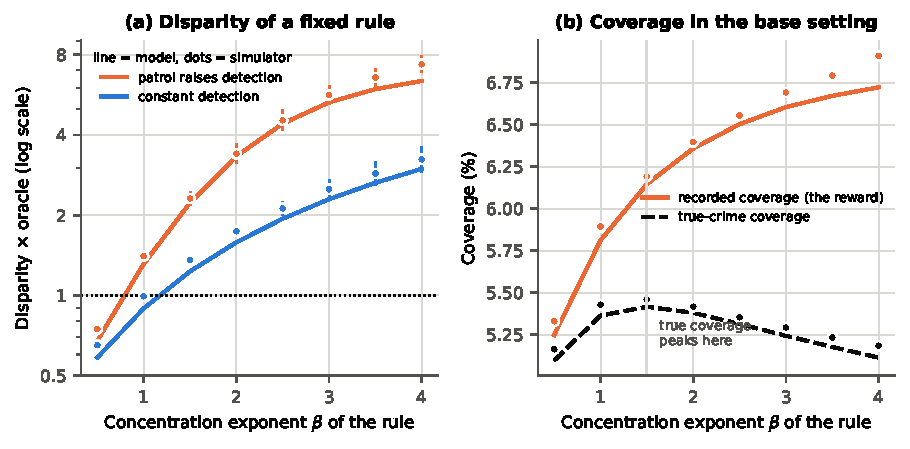
\includegraphics[width=\widefigwidth]{figures/fig_theory.pdf}
\caption{Mean-field model (lines) against the agent-based simulator (dots; bars
= 95\% CI over 6 seeds) for fixed rules with $w=\mu=0$. (a) The recording loop
raises the disparity of the same rule. (b) In the base setting the proxy reward
keeps rising with concentration after true-crime coverage has peaked.}
\label{fig:theory}
\end{widefigure}

\section{Results}

\begin{landtable}
\caption{E1/E4. Disparity relative to the greedy oracle (geometric mean with 95\%
hierarchical-bootstrap CI), raw disparity, coverage of true and recorded crime,
proxy gap and over-recording ratio. Eval seeds 200--229; ``Seeds'' = training
seeds.}
\label{tab:e1}
\begin{fitbox}
\begin{tabular}{lccccccc}
\toprule
Policy & Seeds & $\times$ oracle [95\% CI] & Disparity & True cov. & Rec.\ cov. &
Proxy gap & Q5/Q1 over-rec. \\
\midrule
\tabinput{tables/e1}
\bottomrule
\end{tabular}
\end{fitbox}
\end{landtable}

\subsection{E1: excess concentration at a coverage cost}
Naive PPO's disparity is \nPPOx$\times$ the oracle's (95\% CI
\nPPOxLo--\nPPOxHi; Table~\ref{tab:e1}, Fig.~\ref{fig:e1}) and
\nPPOvsEWMA$\times$ the PredPol heuristic's. The five training seeds range from
\nPPOseedMin$\times$ to \nPPOseedMax$\times$; this instability is part of the
result and is carried by the interval. PPO has the second-highest recorded
coverage of any policy (\nPPOrec, against \nEWMArec{} for PredPol), but its
true-crime coverage (\nPPOlat) is below the oracle's (\nORlat), PredPol's
(\nEWMAlat) and every hotspot baseline. The rule it learns
(Table~\ref{tab:rules}) concentrates sharply on recorded crime
($\beta\approx\nPPObeta$), adds an explicit tilt toward high-hardship districts
($w\approx\nPPOw$) and almost no uniform mix ($\mu\approx\nPPOmu$). The
PredPol heuristic, which uses the same signal without optimising anything, is
at \nEWMAx$\times$: as consequence (i) of Section~\ref{sec:model} predicts, the
loop alone puts a proportional rule above need.

\begin{widefigure}
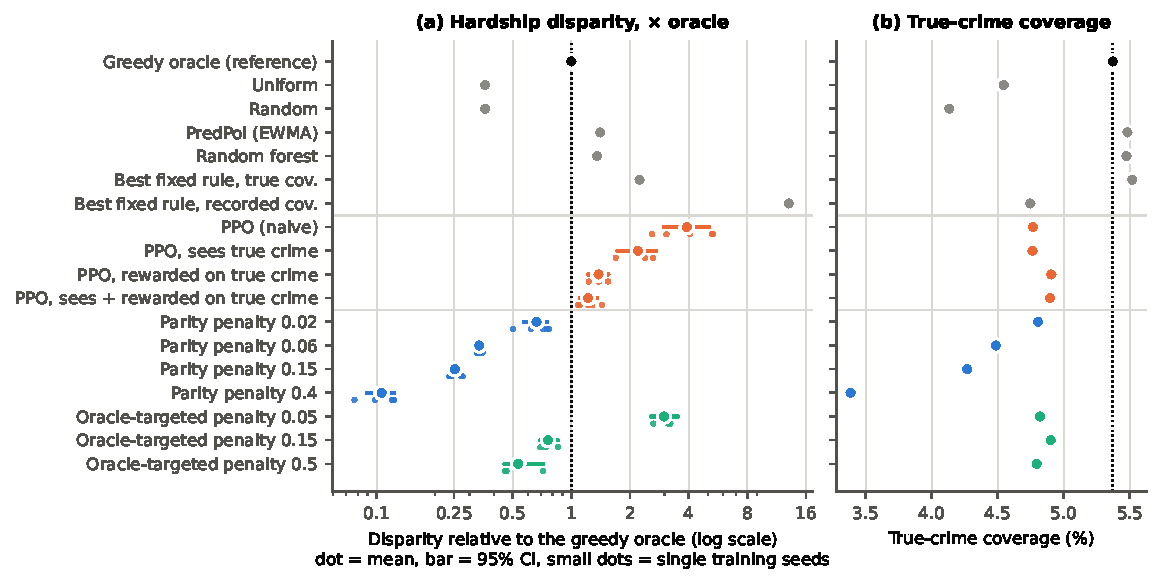
\includegraphics[width=\widefigwidth]{figures/fig_e1_disparity.pdf}
\caption{E1/E4. (a) Disparity relative to the greedy oracle; 1 = need-proportional
patrol. (b) Coverage of true crime; the dotted line is the oracle.}
\label{fig:e1}
\end{widefigure}

\subsection{The bias grows with optimisation, with or without RL}
\label{sec:optim}
\textbf{Exhaustive search.} We searched the same rule class without RL:
192 fixed $(\beta, w, \mu)$ settings scored on seeds 1000--1002, then re-evaluated
on the evaluation seeds. The fixed rule that maximises PPO's own reward reaches a
higher recorded coverage (\nBRRrec{} vs \nPPOrec), so PPO at 400k steps has not
found the optimum of its objective, and it is far more skewed (\nBRRx$\times$
the oracle) with the maximal concentration and hardship tilt the class allows,
as consequence (iii) predicts. The heuristic, the learner and the search thus
line up in the order of how hard they push on the proxy: \nEWMAx$\times$,
\nPPOx$\times$, \nBRRx$\times$.

\textbf{Is PPO simply under-trained?} The gap between PPO's reward and the
fixed-rule optimum invites the objection that the learner is broken and its bias
is noise. We ran three checks (Table~\ref{tab:opt}, Fig.~\ref{fig:opt}).
\emph{Longer training.} Three seeds trained for 1.2M steps with a snapshot every
100k. The reward stops improving by 400k steps (recorded coverage
\nCurveRecStart{} at 100k, \nCurveRecMid{} at 400k, \nCurveRecEnd{} at 1.2M) and
stays below the fixed-rule optimum, so PPO with default settings sits on a
plateau that more steps do not leave. Disparity follows the reward: it rises
from \nCurveXStart$\times$ to \nCurveXMid$\times$ the oracle over the first
400k steps and drifts to \nCurveXEnd$\times$ as the reward slips back. On the 30
evaluation seeds the 1.2M-step policies are at \nLongX$\times$ (95\% CI
\nLongXLo--\nLongXHi), against \nThreeX$\times$ for the same three seeds at 400k.
\emph{Hyper-parameters.} Four variants at 400k steps, three seeds each, change
the learning rate, the entropy bonus and the rollout length. Disparity ranges
from \nHpXMin$\times$ to \nHpXMax$\times$ and no interval comes below
\nHpLoMin$\times$. The variants are ordered by how well they optimise the
proxy: the smaller learning rate and the longer rollouts reach the highest
recorded coverage and the highest disparity, and the larger learning rate
reaches the lowest of both. \emph{Reward against disparity.} Across all \nHpN{}
trained naive models the rank correlation between recorded coverage and log
disparity is \nHpRho{} ($p\nHpRhoP$), and across the \nSnapN{} snapshots of the
long runs it is \nSnapRho. The best-optimised single model reaches a recorded
coverage of \nBestModelRec{} at \nBestModelX$\times$ the oracle, next to the
fixed rule's \nBRRrec{} at \nBRRx$\times$. True-crime coverage barely moves
across these models (\nHpLatMin--\nHpLatMax). Under-optimisation therefore makes
PPO look less biased, not more: the headline \nPPOx$\times$ is what a mediocre
optimiser of this proxy produces, and a better one produces more.

\begin{table}[t]
\caption{Optimisation check. Naive PPO under different training budgets and
hyper-parameters (training seeds 0--2, eval seeds 200--229), and the fixed rule
that maximises the same reward.}
\label{tab:opt}
\centering
\setlength{\tabcolsep}{3pt}
\begin{fitbox}
\begin{tabular}{lcccc}
\toprule
Setting & Seeds & $\times$ oracle [95\% CI] & Recorded cov. & True cov. \\
\midrule
\tabinput{tables/optimisation}
\bottomrule
\end{tabular}
\end{fitbox}
\end{table}

\begin{widefigure}
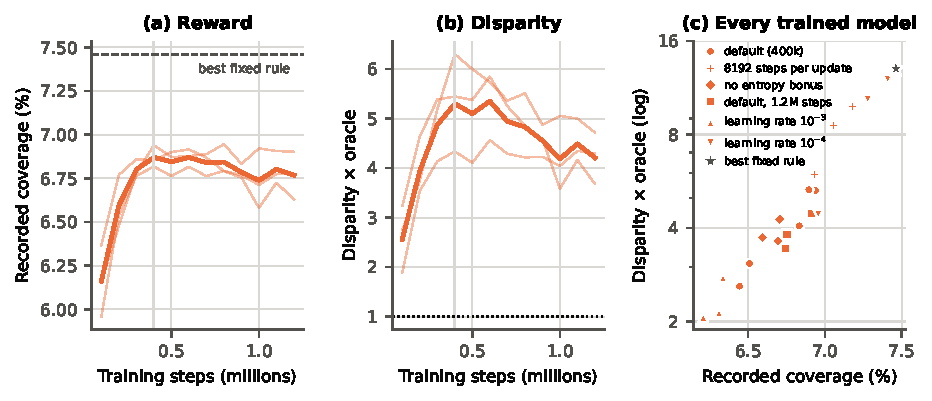
\includegraphics[width=\widefigwidth]{figures/fig_optimisation.pdf}
\caption{Optimisation check. (a) Recorded coverage and (b) disparity relative to
the oracle along 1.2M steps of training (thin lines = training seeds; the
vertical line marks the 400k budget used elsewhere; dashed = best fixed rule).
(c) Every trained naive model: the more reward a model obtains, the more
disparate it is.}
\label{fig:opt}
\end{widefigure}

\begin{table}[t]
\caption{Rule parameters. RL rows: mean action over 5 eval episodes per training
seed, averaged over seeds.}
\label{tab:rules}
\centering
\begin{tabular}{lccc}
\toprule
Policy & $\beta$ & $w$ & $\mu$ \\
\midrule
\tabinput{tables/rules}
\bottomrule
\end{tabular}
\end{table}

\subsection{E2: the policy inflates its own objective}
Naive PPO's proxy gap is \nPPOgap{} -- recorded coverage overstates true
coverage by about two percentage points -- against \nEWMAgap{} for PredPol and
\nORgap{} for the oracle (Table~\ref{tab:e1}). The gap opens in the first shifts
and widens over the episode (Fig.~\ref{fig:e2}a). The records it learns from are
tilted: the top hardship quintile is over-recorded relative to the bottom one by
a factor of \nPPOrd, against \nORrd{} for the oracle. We also computed a
self-induced signal (the partial correlation between last shift's patrol and this
shift's over-recording). It is high for every targeted policy (PPO \nPPOsis,
oracle \nORsis, PredPol \nEWMAsis), so it measures the strength of the detection
channel rather than a policy-specific loop, and we do not use it as evidence. We
likewise drop the ``runaway index'' of our earlier draft: a static allocation
with no feedback scores 1.0 on it.

\begin{widefigure}
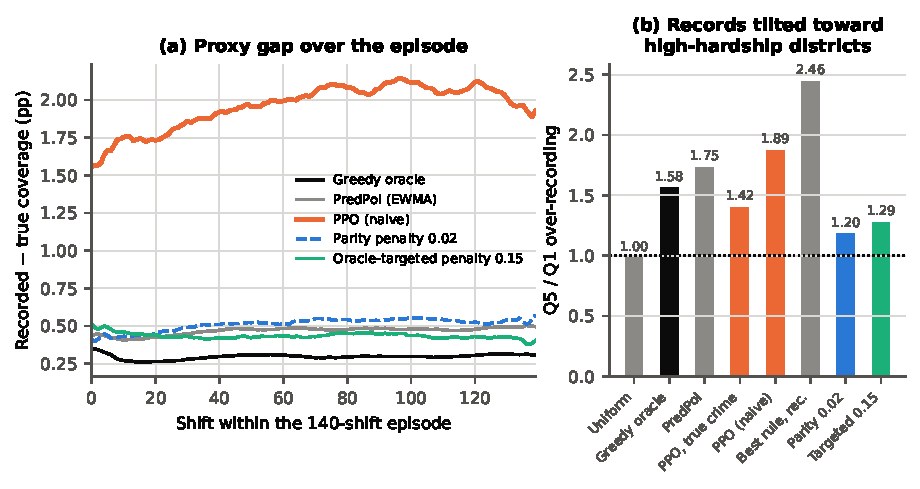
\includegraphics[width=\widefigwidth]{figures/fig_e2_contamination.pdf}
\caption{E2. (a) Recorded minus true coverage over the episode, mean over
evaluation episodes. (b) Over-recording of the top hardship quintile relative to
the bottom one; 1 = records are not tilted.}
\label{fig:e2}
\end{widefigure}

\subsection{E3: excess on disadvantaged districts, beyond need}
For every (episode, shift, district) after a 30\% burn-in we regress the
\emph{allocation residual} $a_r - n_r$ on standardised hardship, need and
poverty, where the need $n_r$ is the district's long-run latent-crime share under
uniform patrol on the same evaluation seeds. Standard errors are clustered on
episode, and a seed-level bootstrap resamples per-training-seed coefficients
(Table~\ref{tab:e3}). The coefficient is descriptive, not causal. Naive PPO's
hardship coefficient is $+\nPPOcoef\times10^{-3}$ per standard deviation
($t=\nPPOt$; seed-level 95\% CI \nPPOcoefLo--\nPPOcoefHi; positive in
\nPPOseedsPos{} seeds), while the oracle and the hotspot baselines show none.
Fig.~\ref{fig:e3} shows the shape: PPO gives the most disadvantaged quintile
\nPPOqfive{} percentage points of patrol share beyond need and takes it from the
middle quintiles (down to \nPPOqtwothree{} points). The proxy-maximising fixed
rule has the same sign and is larger ($+\nBRRcoef\times10^{-3}$). This is
about a quarter of the effect our earlier draft reported ($+0.017$ with
$p<10^{-300}$), which controlled only for the current shift's latent share and
treated region-shifts as independent.

\begin{table}[t]
\caption{E3. Hardship coefficient on the allocation residual
($\times10^{-3}$ per s.d.), episode-clustered $t$, seed-level bootstrap CI and
the number of training seeds with a positive coefficient.}
\label{tab:e3}
\centering
\setlength{\tabcolsep}{3pt}
\begin{fitbox}
\begin{tabular}{lcccc}
\toprule
Policy & Coef. & $t$ & Seed CI & $>0$ \\
\midrule
\tabinput{tables/e3}
\bottomrule
\end{tabular}
\end{fitbox}
\end{table}

\begin{figure}[t]\centering
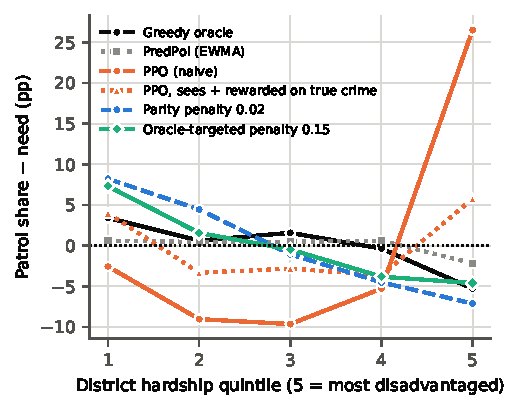
\includegraphics[width=\narrowfigwidth]{figures/fig_e3_need_residual.pdf}
\caption{E3. Patrol share minus latent need, summed within each hardship
quintile (after a 30\% burn-in).}
\label{fig:e3}
\end{figure}

\subsection{Attribution: reward or observation?}
Table~\ref{tab:attr} crosses what PPO observes with what it is rewarded on.
Rewarding true-crime coverage while still observing only recorded crime cuts the
excess from \nAttRecRec$\times$ to \nAttRecLat$\times$; letting the policy observe
true crime while still rewarding recorded coverage cuts it only to
\nAttLatRec$\times$. Both together give \nAttLatLat$\times$, still above the
oracle because the rule reads recorded crime. The reward is the larger lever,
which is what consequence (iii) says: the excess is asked for by the objective,
not caused by missing information.

\begin{table}[t]
\caption{$2\times2$ attribution, $\times$ oracle [95\% CI], training seeds
0--2.}
\label{tab:attr}
\centering
\setlength{\tabcolsep}{4pt}
\begin{tabular}{lcc}
\toprule
& \multicolumn{2}{c}{Rewarded on} \\
Observes & recorded crime & true crime \\
\midrule
\tabinput{tables/attribution}
\bottomrule
\end{tabular}
\end{table}

\subsection{E4: penalties overcorrect; a targeted penalty does better}
A penalty on raw disparity pushes $\delta$ toward 0, not toward need. Every
parity weight lands \emph{below} the oracle -- \nPtwox$\times$ at the lightest
($w=0.02$) and \nPfourx$\times$ at the heaviest -- and E3 coefficients turn
negative (\nPtwoCoef$\times10^{-3}$ at $w=0.02$): disadvantaged districts end up
under-patrolled relative to need, and true-crime coverage falls to \nPfourlat{}
at $w=0.4$. The oracle-targeted penalty charges only for disparity above the
reference. At $w=0.15$ it reaches \nRonefivex$\times$ the oracle (95\% CI
\nRonefiveLo--\nRonefiveHi), the closest of any learned policy, and raises
true-crime coverage above naive PPO's (\nRonefivelat{} vs \nPPOlat; Holm
$p=\nRonefiveLatP$). It does not hit the target exactly: $w=0.05$ is too weak
(\nRfivex$\times$) and $w=0.5$ lands at \nRhalfx$\times$ (Fig.~\ref{fig:e4}).
As a check on the form of the constraint, a Lagrangian PPO that holds
disparity at the oracle's level by dual ascent (ceiling 2.78, 3 seeds) also
reaches the target, \nLagX$\times$ the oracle (95\% CI \nLagXLo--\nLagXHi), but
at a lower true-crime coverage (\nLagLat) than the oracle-targeted penalty.

\begin{figure}[t]\centering
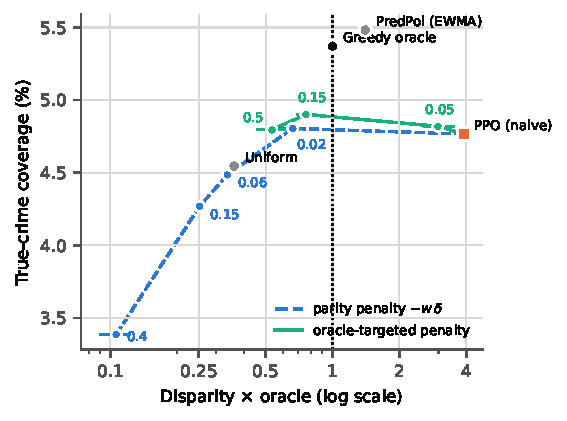
\includegraphics[width=\narrowfigwidth]{figures/fig_e4_frontier.pdf}
\caption{E4. True-crime coverage against disparity relative to the oracle for the
two penalty families (labels = weight $w$; bars = 95\% CI).}
\label{fig:e4}
\end{figure}

\subsection{E5: removing the detection channel}
We retrain PPO and the parity-penalised agent ($w=0.06$) in two settings where
patrol no longer changes detection, each scored against its own oracle
(Table~\ref{tab:e5}, Fig.~\ref{fig:e5}). \emph{Perfect observation} sets $q_r=1$:
it removes the action-dependence but also raises the volume of recorded crime and
makes the reward equal to true coverage. \emph{Constant detection} sets
$q_r=0.667$ for every district, the uniform-patrol rate, so the volume of data is
unchanged and only the dependence on patrol is removed. PPO's excess drops from
\nEfiveBase$\times$ (\nEfiveBaseLo--\nEfiveBaseHi) to \nEfivePerf$\times$ and
\nEfiveConst$\times$ (\nEfiveConstLo--\nEfiveConstHi) respectively, and
over-recording drops to 1. The constant-detection control shows the reduction is
due to the detection channel, not to more data.

The residual of about 1.5$\times$ is what the model of Section~\ref{sec:model}
predicts rather than an optimisation artefact. Without contamination the reward
equals true coverage up to a constant, and true coverage is nearly flat in the
rule's concentration: fixed rules with $\beta$ anywhere from 1.5 to 4 come
within \nThConstFlat\% of the best coverage, about one standard error, while
their disparity ranges from \nThConstBetaOneFiveX$\times$ to
\nThSimConstFour$\times$ the oracle (Fig.~\ref{fig:theory}a). A coverage maximiser has no reason to be
need-proportional even when its data are clean; contamination is what turns that
modest excess into a large one. The parity-penalised agent sits at
\nEfiveFairMin--\nEfiveFairMax$\times$ in every setting. This is
mechanism-isolating evidence within the simulator's structural equations, not
proof of a causal effect in real policing.

\begin{table}[t]
\caption{E5. Oracle disparity and $\times$ own-setting oracle [95\% CI] for
naive and parity-penalised PPO, and PPO's over-recording ratio. 3 training seeds,
eval seeds 300--319.}
\label{tab:e5}
\centering
\setlength{\tabcolsep}{3pt}
\begin{fitbox}
\begin{tabular}{lcccc}
\toprule
Setting & Oracle & PPO & Penalised & Over-rec. \\
\midrule
\tabinput{tables/e5}
\bottomrule
\end{tabular}
\end{fitbox}
\end{table}

\begin{figure}[t]\centering
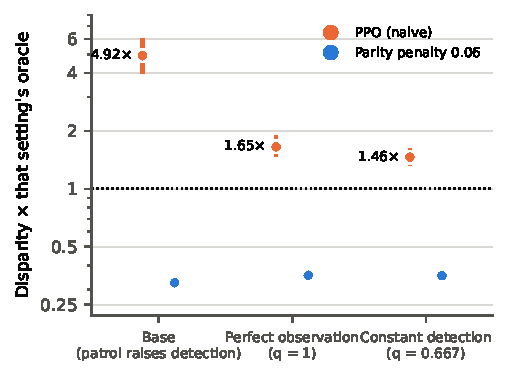
\includegraphics[width=\narrowfigwidth]{figures/fig_e5_interventions.pdf}
\caption{E5. Disparity relative to each setting's own greedy oracle (bars = 95\%
CI).}
\label{fig:e5}
\end{figure}

\subsection{Sensitivity to the uncalibrated parameters}
\label{sec:sens}
The strength of the loop depends on detection and deterrence parameters that are
not calibrated to data. We retrained naive PPO (3 seeds, 400k steps) with each
of them moved in both directions, and once without the socio-economic inputs,
and compared each policy with the oracle of its own setting
(Table~\ref{tab:sens}, Fig.~\ref{fig:sens}). PPO exceeds the oracle in every
setting, from \nSensMin$\times$ to \nSensMax$\times$, and the smallest lower
confidence bound is \nSensLoMin$\times$. The size of the excess moves as
Eq.~\eqref{eq:eps} predicts. Lower baseline reporting and weaker deterrence
raise the elasticity of the recorded signal ($\varepsilon=\nEpsLowPReport$ and
$\nEpsWeakDeterrence$) and give the largest excess (\nSensLowPReport$\times$ and
\nSensWeakDeterrence$\times$); higher baseline reporting and a smaller detection
gain lower it ($\nEpsHighPReport$ and $\nEpsLowDetectGain$) and give the
smallest (\nSensHighPReport$\times$ and \nSensLowDetectGain$\times$). Over the
base setting and the six parameter variants the rank correlation between
$\varepsilon$ and the log excess is \nSensRho{} ($p=\nSensRhoP$). The fit is not
exact: stronger deterrence lowers $\varepsilon$ to $\nEpsStrongDeterrence$ but
the excess (\nSensStrongDeterrence$\times$) is not below the base setting's
(\nSensBase$\times$), although the intervals overlap. Where $\varepsilon$ is
close to zero PPO is still about three times the oracle, in line with E5: a
coverage maximiser concentrates even when the record does not respond to it.
Removing the socio-economic inputs changes little (\nSensNoSocioObs$\times$), so
the policy does not need hardship indicators to produce the skew; recorded crime
carries it.

\begin{table}[t]
\caption{Sensitivity. Elasticity of the recorded signal at proportional patrol
(Eq.~\eqref{eq:eps}), oracle disparity, naive PPO $\times$ own-setting oracle
[95\% CI], proxy gap in percentage points and over-recording ratio. Base values:
detection gain 0.55, baseline reporting 0.30, deterrence slope 0.26. 3 training
seeds, eval seeds 300--319.}
\label{tab:sens}
\centering
\setlength{\tabcolsep}{3pt}
\begin{fitbox}
\begin{tabular}{lccccc}
\toprule
Setting & $\varepsilon$ & Oracle & PPO $\times$ oracle & Gap & Over-rec. \\
\midrule
\tabinput{tables/sensitivity}
\bottomrule
\end{tabular}
\end{fitbox}
\end{table}

\begin{figure}[t]\centering
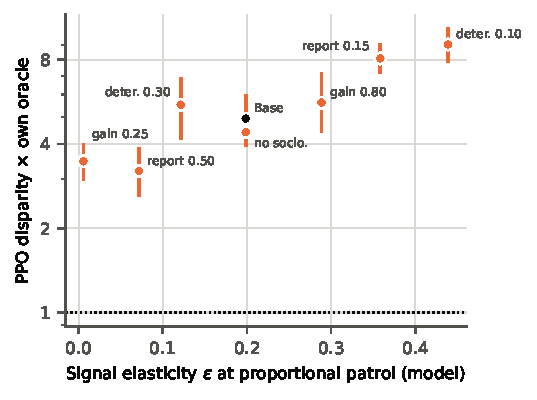
\includegraphics[width=\narrowfigwidth]{figures/fig_sensitivity.pdf}
\caption{Sensitivity. Naive PPO's disparity relative to its own oracle against
the model's signal elasticity in each setting (bars = 95\% CI).}
\label{fig:sens}
\end{figure}

\subsection{Robustness to the choice of reference}
\label{sec:reference}
Section~\ref{sec:measure} showed that orderings and contrasts cannot depend on
the reference. Table~\ref{tab:ref} shows how the \emph{level} moves when the
greedy oracle is replaced by Uniform patrol, by the PredPol-like rule
$(1,0,0)$, or by the fixed rule with the highest true-crime coverage. PPO is
above every one of them: \nRefUniPPO$\times$ Uniform, \nRefEwmaPPO$\times$ the
PredPol-like rule and \nRefBrlPPO$\times$ the coverage-optimal rule. The last
comparison matters most: PPO is more concentrated than the allocation that
would maximise true-crime coverage, so its excess cannot be defended as
efficient targeting.

Two measures need no reference policy. The \emph{top-quintile excess} is the
patrol share of the most disadvantaged quintile divided by its share of latent
crime (1 = in proportion to true crime). It is \nTopPPO{} for PPO (95\% CI
\nTopPPOLo--\nTopPPOHi), \nTopBRR{} for the proxy-maximising rule, \nTopEWMA{}
for PredPol, \nTopOR{} for the oracle and \nTopTarget{} for the oracle-targeted
penalty; Uniform patrol under-serves that quintile (\nTopUNI). The
total-variation distance between patrol shares and latent-crime shares over all
22 districts tells the same story (\nTvPPO{} for PPO against \nTvOR{} for the
oracle), and shows that parity is as far from need as naive PPO is, in the
opposite direction.

\begin{table}[t]
\caption{Reference robustness. Disparity relative to four reference policies
(geometric mean of paired ratios), and two reference-free measures:
top-quintile patrol share over latent-crime share, and total-variation distance
between patrol and latent-crime shares.}
\label{tab:ref}
\centering
\setlength{\tabcolsep}{3pt}
\begin{fitbox}
\begin{tabular}{lcccccc}
\toprule
& \multicolumn{4}{c}{$\times$ reference} & \multicolumn{2}{c}{Reference-free} \\
\cmidrule(lr){2-5}\cmidrule(lr){6-7}
Policy & Oracle & Uniform & PredPol-like & Best true cov. & Top excess & TV \\
\midrule
\tabinput{tables/reference}
\bottomrule
\end{tabular}
\end{fitbox}
\end{table}

\begin{widetable}
\caption{Pre-specified paired contrasts. For disparity, the ratio of geometric
means; for coverage, the difference in percentage points. Two-sided bootstrap
$p$-values, Holm-adjusted over all \nNContrasts{} rows.}
\label{tab:contrasts}
\begin{fitbox}
\begin{tabular}{llccc}
\toprule
Contrast & Metric & Estimate & 95\% CI & $p_{\mathrm{Holm}}$ \\
\midrule
\tabinput{tables/contrasts}
\bottomrule
\end{tabular}
\end{fitbox}
\end{widetable}

\section{Discussion}

The naive policy is not failing at its task. Given a reward for covering recorded
crime, concentrating on recorded hotspots is the right answer, and the model
shows why the right answer is extreme: the proxy is linear in the allocation and
the record moves in the optimiser's favour. The heuristic, the learner and the
exhaustive search differ only in how far along that slope they get. Framing the
result as ``RL is biased'' would therefore be wrong in a way that matters for
practice, because it suggests a better learner as the remedy; a better learner
is worse. What has to change is the objective, and the two levers we tested act
on it directly. Rewarding an estimate of true coverage removes most of the
excess even when the agent still sees only recorded crime. And an equity
constraint should be referenced to need rather than to parity: parity penalties
under-patrol the districts with the most crime, while a penalty anchored at the
need-proportional reference approaches it and improves true coverage.

The model also says when the problem is mild. The loop's multiplier is
$1/(1-\beta\varepsilon)$, so the excess is governed by the elasticity of the
record to patrol, a quantity that could in principle be estimated from
deployment experiments without knowing latent crime. Where records
come mainly from victim reports and depend little on patrol presence,
$\varepsilon$ should be near or below zero and the loop benign; where records
are mostly officer-initiated, as for the drug offences studied by Lum and
Isaac~\cite{lum2016}, it should be large.

\textbf{Limitations.}
(1)~The claims concern a simulated world with parametric deterrence and detection
that are not calibrated to an external estimate of reporting rates; the
sensitivity analysis (Section~\ref{sec:sens}) varies them but does not replace
calibration.
(2)~Quintiles of 22 districts hold only 4--5 districts each.
(3)~Training is unstable across seeds (\nPPOseedMin--\nPPOseedMax$\times$ for
naive PPO); we report the spread and carry it in every interval, and E5 rests on
3 training seeds. Section~\ref{sec:optim} shows that the spread tracks how much
reward each run obtains, and that default PPO does not reach the optimum of its
objective.
(4)~Policies act through a three-parameter rule. This is what makes exhaustive
search and the closed-form analysis possible, but a richer action space could
behave differently.
(5)~Residential population is uniform across districts.
(6)~The reference is normative, not optimal: need-proportional patrol is not the
coverage-maximising allocation.
(7)~Offenders do not adapt to patrol.
(8)~The mean-field model ignores count noise and the within-episode transient;
it is accurate here but need not be for much smaller crime counts.

\section{Conclusion}
In a crime simulator whose latent process is known, optimising coverage of
recorded crime concentrates patrol well beyond a need-proportional reference
-- \nPPOx$\times$ for an RL agent and \nBRRx$\times$ for the exact optimum of
the same objective -- while covering less true crime than simple heuristics and
over-patrolling disadvantaged districts beyond their need. A mean-field model
attributes this to the positive elasticity of the record to patrol, which
multiplies a rule's tilt by $1/(1-\beta\varepsilon)$ and moves the proxy optimum
away from the true one. Removing the patrol-dependence of detection removes most
of the excess, the reward is a larger lever than the observation, and a penalty
targeted at need rather than parity gets closest to the reference. The same
pattern -- an optimiser pursuing a signal it contaminates -- applies wherever
actions decide what gets observed.


\section*{Acknowledgment}
We thank PES University and the Department of Computer Science and Engineering
(AI \& ML). This work was carried out as Capstone Project Phase 2 (UE23AM320B).

\bibliographystyle{IEEEtran}
\bibliography{refs}

\end{document}
